\documentclass[10pt,landscape]{article}
\usepackage{multicol}
\usepackage{calc}
\usepackage{ifthen}
\usepackage[landscape]{geometry}
\usepackage{amsmath,amsthm,amsfonts,amssymb}
\usepackage{color,graphicx,overpic}
\usepackage{hyperref}
\usepackage{matlab-prettifier}
\usepackage{listings}
\usepackage[utf8]{inputenc}


\pdfinfo{
  /Title (ebv-zusammendaffung.pdf)
  /Creator (Michael Blättler)
  /Author (Michael Blättler)
  /Subject (EBV)
  /Keywords (EBV, HSLU)}

% This sets page margins to 1cm
\geometry{top=1cm,left=1cm,right=1cm,bottom=1cm}

\DeclareMathSymbol{*}{\mathbin}{symbols}{"01}

% Turn off header and footer
\pagestyle{empty}

% Redefine section commands to use less space
\makeatletter
\renewcommand{\section}{\@startsection{section}{1}{0mm}%
                                {-1ex plus -.5ex minus -.2ex}%
                                {0.5ex plus .2ex}%x
                                {\normalfont\large\bfseries}}
\renewcommand{\subsection}{\@startsection{subsection}{2}{0mm}%
                                {-1explus -.5ex minus -.2ex}%
                                {0.5ex plus .2ex}%
                                {\normalfont\normalsize\bfseries}}
\renewcommand{\subsubsection}{\@startsection{subsubsection}{3}{0mm}%
                                {-1ex plus -.5ex minus -.2ex}%
                                {1ex plus .2ex}%
                                {\normalfont\small\bfseries}}
\makeatother

% Define BibTeX command
\def\BibTeX{{\rm B\kern-.05em{\sc i\kern-.025em b}\kern-.08em
    T\kern-.1667em\lower.7ex\hbox{E}\kern-.125emX}}

% Don't print section numbers
\setcounter{secnumdepth}{0}


\setlength{\parindent}{0pt}
\setlength{\parskip}{0pt plus 0.5ex}

% -----------------------------------------------------------------------

\graphicspath{ {images/} }

\begin{document}
\lstset{style=Matlab-editor}

\raggedright
\footnotesize
\begin{multicols}{3}


% multicol parameters
% These lengths are set only within the two main columns
%\setlength{\columnseprule}{0.25pt}
\setlength{\premulticols}{1pt}
\setlength{\postmulticols}{1pt}
\setlength{\multicolsep}{1pt}
\setlength{\columnsep}{2pt}

\begin{center}
     \Large{\underline{HSLU T\&A: EBV}} \\
\end{center}

\section{Einführung}
\subsection{Sensoren}
\begin{description}
    \item[CCD] Beim CCD-Sensor wird der photoelektrische Effekt ausgenutzt. Dabei wird bei Wellenlängen über 1'100 nm (IR) Elektronen-Lochpaare erzeugt. Die Anzahl dieser Paare ist proportional zur Intensität des einfallenden Lichtes. Dies wird vom CCD-Sensor in elektrische Spannung umgewandelt.\\
    Um die Daten auszulesen, werden diese aus dem Sensor herausgeschoben (Siehe Abbildung 13 im Skript S. 9). Dies nennt sich das ''Eimerkettenprinzip''.
    \item[CMOS] Der CMOS Sensor funktioniert grundsätzlich identisch wie der CCD-Sensor. Beim CMOS-Sensor hat jedoch jedes Pixel einen eigenen Verstärker samt Auswertungslogik. Der hohe Platzbedarf sowie das hohe Pixelrauschen sprachen lange gegen die CMOS Sensoren, obwohl diese sonst viel Vorteile haben. So haben diese einen geringeren Stromverbrauch, kleineres Übersprechen bei hohen Belichtungsstärken (Blooming-Effekt) und durch den Einsatz eines separaten Verstärkers für jedes Pixel besteht die Möglichkeiten einer logarithmischen Messung der Belichtungsstärke.
\end{description}
\subsection{Rasterung}
Die Rasterung oder räumliche Auflösung ist ein Mass für die Detailtreue eines Bildes.\\
Zwischen der Gegenstands- (g), Bildweite (b) und Brennweite (f) besteht folgender Zusammenhang:
\begin{equation}
\frac{1}{g} + \frac{1}{b} = \frac{1}{f}
\end{equation}
\begin{equation}
b=\frac{f\cdot g}{g - f}
\end{equation}
Weiterhin folgt aus dem Strahlensatz der direkte Zusammenhang zwischen Gegenstands- (G) und Buildgrösse (B).
\begin{equation}
\frac{B}{G}=\frac{b}{g}
\end{equation}
Beispielrechnung Skript S.14.


\section{Punktoperation und Bildverknüpfungen}
Bei den Punktoperationen wird jedes Pixel isoliert betrachtet und unabhängig von seinen Nachbarpixel verändert.
\subsection{Transformationstabellen}
Es wird grundsätzlich zwischen zwei verschiedenen Arten unterschieden:
\begin{description}
    \item[Homogene Punktoperationen] Bei diesen Operationen spielt die Position des Pixels keine Rolle für die angewendete Transformation.\\
    Bsp. Invertiertes Bild
    \item[inhomogene Punktoperationen] Bei dieser Art von Operationen wird die Position des Pixels für die Transformation berücksichtigt.\\
    Bsp. Farbverlauf
\end{description}

\subsubsection{Lineare Grauwerttransformationen}
Beispiele sind: \textbf{Spreizung} und \textbf{inverses Bild}\\
Für lineare Transformationen werden oft LUT (Look up tables) verwendet.
\begin{lstlisting}
%LUT for inverse image
LUT_Inv = uint8([255:-1:0]);

% LUT for spreading (Spreizung)
LUT_Spread = uint8(((0:255)-50) * 2);

%apply LUT
ImageInv = intlut(Image, LUT_xx);
\end{lstlisting}

\subsubsection{Nichtlineare Grauwerttransformationen (Gammakorrektur)}
Wichtigstes Beispiel: \textbf{Gammakorrektur}
Die Gammakorrektur ist eine häufig verwendete Korrekturfunktion zur Überführung einer physikalisch proportional (d. h. linear) wachsenden Grösse in eine dem menschlichen Empfinden gemäss nicht linear wachsende Grösse.

\subsection{Histogrammausgleich}
Der Histogrammausgleich versucht den zur Verfügung stehenden Grauwertbereich optimal auszunutzen. Dabei sollte jeder Grauwert gleichmässig auftreten.
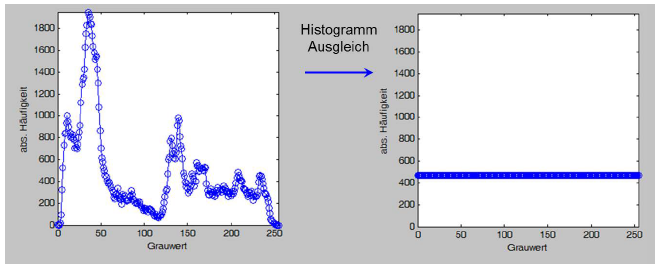
\includegraphics[width=\textwidth/3]{histogrammausgleich.PNG}
\begin{lstlisting}
[Hist, Val] = imhist(Image);

CumHist = cumsum(Hist)/sum(Hist);
% remark: cumsum()
% Addiert alle Ellemente von 0 bis i.

%do the histogram equalization
%LUT for histogram equalization
LUT_Equ = uint8(CumHist*255);

%apply LUT
ImageEqu = intlut(Image, LUT_Equ);
\end{lstlisting}

\subsection{Motiondetektion durch Differenzbildung}
Durch Substraktion von zwei Bildern kann die Veränderung zwischen den Bildsequenzen erkennt werden.
\begin{lstlisting}
%this is the delta of the step
Delta = 2;

%read first image to index 0
Index = 0;
FileName = strcat(Path, sprintf('%04d', Index), '.bmp');
ImageOld = imread(FileName);
%loop over required range, with step size Delta
for Index = Delta:Delta:400
    %read next image
    FileName = strcat(Path, sprintf('%04d', Index), '.bmp');
    ImageAct = imread(FileName);
    
    %this is the threshold value (chosen manually)
    Threshold = 15;
    
    %calcuate difference image
    DiffImage = uint8((255+double(ImageAct)-double(ImageOld))/2);
    %remark:
    %DiffImage = ImageAct-ImageOld; would cause the same effect
    %but the image would be darker. The factors are for normalization
    %purposes

    %calculate the threshold image
    ThreshImage = (abs(128-DiffImage) > Threshold) * 255;
    
   %plot the images
    pause(0.1);
end
\end{lstlisting}
\subsubsection{Gleitendes Mittel}
Ziel des gleitenden Mittels ist es, eine möglich genaue Hypothese des unbeweglichen Hintergrundbildes zu erhalten.\\
Die geschieht über folgende Gleichung:
\begin{equation}
    B_k = \alpha * B_{k-1} + (1-\alpha) * I_k
\end{equation}
Diese kann als Tiefpassfilter für jedes Pixel über die Zeit interpretiert werden.\\
Um zu Berechnen wie viele Integrationen (Bilder) es benötigt, bis stationäre Änderungen verschwunden sind, kommt folgende Formel zur Verwendung.
\begin{equation}
    n=\frac{\log(0.1)}{\log(\alpha)}
\end{equation}
\begin{lstlisting}
    %estimate new background as sliding average
    BackGround =  uint8(alpha*double(BackGround) +(1-alpha)*double(ImageAct));
\end{lstlisting}
\subsubsection{Statische Analyse zur Hintergrundschätzung}
Die statische Analyse ist die heutige ''State-of-the-Art'' Implementierung der Hintergrundabschätzung. Sie benutzt statistische Werte wie \textit{Mittelwert} und \textit{Varianz} um das Hintergrundbild zu schätzen.\\
Dabei wird von jedem Pixel der Mittelwert bestimmt und über die Varianz und einem vordefinierten Schwellwert analysiert, ob sich dieses Pixel verändert hat oder nicht.\\
Wird auch \textbf{Gaussian Mixture Model} bezeichnet.
\section{Filteroperationen}
Bei Filteroperationen werden neu auch die Werte der Nachbarpixel in Betracht gezogen.\\
Es gibt folgende Filtertypen:
\begin{description}
    \item[homogene Filter] Die Berechnung der Transformation $f(g)$ wird für jedes Pixel unabhängig von dessen Position vorgenommen.
    \item[inhomogene Filter] Die Berechnung der Transformation $f(g)$ hängt explizit von der Position des Pixels im Bild ab.
    \item[lineare Filter] Die Berechnung der Transformation $f(g)$ hängt für jedes Pixel linear von $g=I_{m,n}$ und den Werten der Nachbarpixel $I_{p,q}$ ab.
    \item [nicht lineare Filter] Identisch mit den linearen Filtern, aber die Abhängigkeit zu den Pixeln ist nicht linear.
\end{description}

\subsection{Lineare Filter}
Lineare Filter werden durch eine Faltung (\ref{eq:conv}) oder Korrelation(\ref{eq:corr}) angewendet.
\begin{equation} \label{eq:conv}
I \otimes h: I_{m,n} \to \sum_{p=-u}^{u}\sum_{q=-v}^{v}I_{m-p,n-q} * h_{p,q}
\end{equation}
\begin{equation} \label{eq:corr}
I \otimes h: I_{m,n} \to \sum_{p=-u}^{u}\sum_{q=-v}^{v}I_{m+p,n+q} * h_{p,q}
\end{equation}
\subsubsection{Tiefpass (Glättung)}
Beim Glätten von Bildern wird durch eine Mittlung der Nachbarpixeln erreicht.\\
Bsp: $R=\frac{1}{9}*\begin{bmatrix}
1 & 1 & 1 \\
1 & 1 & 1 \\
1 & 1 & 1
\end{bmatrix}$
oder $G=\frac{1}{16}*\begin{bmatrix}
1 & 2 & 1 \\
2 & 4 & 2 \\
1 & 2 & 1
\end{bmatrix}$
\begin{lstlisting}
%u3 Glaettung
%apply a filter of size 2x2
R = 1/4*[1 1; 1 1];
Image1 = uint8(imfilter(double(Image), R));
\end{lstlisting}
\subsubsection{Hochpass (Kantenhervorhebung)}
Bei der Kantenhervorhebung werden Abweichungen zu den benachbarten Pixel signalisiert.\\
Dafür wird die Ableitung der Pixel eruiert (Herleitung Skript S.37).
\begin{equation}
\frac{\partial I}{\partial x}=\frac{I_{m,n+1}-I_{m,n-1}}{2} \to h_x = \frac{1}{2}*
\begin{bmatrix}
-1 & 0 & 1
\end{bmatrix}
\end{equation}
\begin{equation}
\frac{\partial I}{\partial y}=\frac{I_{m+1,n}-I_{m-1,n}}{2} \to h_y = \frac{1}{2}*
\begin{bmatrix}
-1 \\
0 \\
1
\end{bmatrix}
\end{equation}
Die obigen Filter $h_x$ und $h_y$ sind sehr fehleranfällig auf Bildrauschen. Durch die Faltung mit Glättungsfiltern kann dieses Rauschen aber reduziert werden.\\
Dies führt zu den Sobel und Prewitt Filter:
\begin{equation*}
Prewitt-Filter: h_x = \begin{bmatrix}
-1 & 0 & 1 \\
-1 & 0 & 1 \\
-1 & 0 & 1
\end{bmatrix}
h_y = \begin{bmatrix}
-1 & -1 & -1 \\
0 & 0 & 0 \\
1 & 1 & 1
\end{bmatrix}
\end{equation*}
\begin{equation*}
Sobel-Filter: h_x = \begin{bmatrix}
-1 & 0 & 1 \\
-2 & 0 & 2 \\
-1 & 0 & 1
\end{bmatrix}
h_y = \begin{bmatrix}
-1 & -2 & -1 \\
0 & 0 & 0 \\
1 & 2 & 1
\end{bmatrix}
\end{equation*}
\begin{lstlisting}
%u3 Gradient1
% Prewitt Filter
DX = [-1 0 1; -1 0 1; -1 0 1];
DY = DX';	
%apply the DX and DY filter
ImageDx = imfilter(Image, DX);
ImageDy = imfilter(Image, DY);
\end{lstlisting}
oder mit den Matlab Funktionen:
\begin{lstlisting}
%u3 Gradient2
%choose the filters
DX = fspecial('sobel')';
DY = fspecial('sobel');
%bzw
DX = fspecial('prewitt')';
DY = fspecial('prewitt');
%apply the DX and DY filter
ImageDx = imfilter(Image, DX);
ImageDy = imfilter(Image, DY);
\end{lstlisting}
\subsubsection{Bestimmen des Steigungswinkel}
Durch Trigonometrie kann die Richtung/Winkel der Steigung evaluiert werden.
\begin{equation}
\alpha = \arctan{\frac{\frac{\partial I}{\partial y}}{\frac{\partial I}{\partial x}}}
\end{equation}
\begin{lstlisting}
%u3 Gradient2
%determine the angle
%(atan2 gives back the whole interval
%]-pi , pi[ )
Angle = atan2(ImageDy, ImageDx);
\end{lstlisting}
\subsubsection{Bildschärfung}
Um ein Bild zu schärfen kann der Laplace Operator verwendet werden. Dieser ist als Summe der zweiten Ableitungen definiert (Herleitung Skript S 38):
\begin{equation}
\Delta I = L = \frac{\partial ^2I}{\partial x^2} + \frac{\partial ^2I}{\partial x^2} \to L = \begin{bmatrix}
0 & -1 & 0 \\
-1 & 4 & -1 \\
0 & -1 & 0
\end{bmatrix}
\end{equation}
In der Bildverarbeitung wird der Laplace Operator wie folgt eingesetzt:
\begin{equation}
1*I+\beta * L
\end{equation}
Wobei der Term $1*I$ benötigt wird, damit das Bild in die Berechnung hineingezogen wird (L alleine detektiert nur die Kanten). Der Faktor $\beta$ beschreibt wie stark das Bild geschärft werden soll.
\begin{lstlisting}
%u3 Bildschaerfung
%define the filter
Beta = 0.5;
Mask = [0 0 0; 0 1 0; 0 0 0] + Beta*[0 -1 0; -1 4 -1; 0 -1 0]
%apply the filter
ImageEnh = imfilter(Image, Mask);
\end{lstlisting}

\subsection{Nichtlineare Filter}
\subsubsection{Median Filter}
Der Median-Filter hilft beim entfernen von Bildstörungen oder beim finden von lokalen Maximas und Minimas.
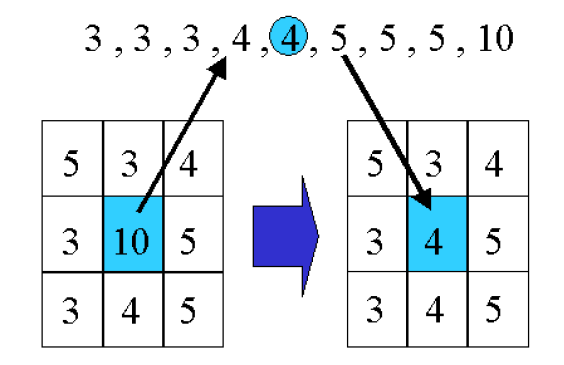
\includegraphics[width=\textwidth/3]{medianfilter.PNG}
\begin{lstlisting}
%u4 MedianFilter
% 5 means take the 5th element in the value order
ImageMedian = ordfilt2(ImageNoise, 5, ones(3,3));
\end{lstlisting}
\subsubsection{Minimas und Maximas}
\begin{lstlisting}
%u4 LocalMaxMin
%apply min/max filter
MinVal = ordfilt2(ImgValley, 1, ones(SizeRegion));
MaxVal = ordfilt2(ImgHill, SizeRegion^2, ones(SizeRegion));

%find local min/max values
LocMin = (MinVal == ImgValley);
LocMax = (MaxVal == ImgHill);
\end{lstlisting}

\section{Morphologische Operationen}
Bei morphologischen Operationen werden die Pixel auf eine bestimmte Struktur hin untersucht.\\
Folgende Operationen sind dabei typisch:
\begin{itemize}
    \item Löschen kleiner Objekte (z.B. Pixelrauschen)
    \item Schliessen von Löchern in Objekten
    \item Zusammenfassen von räumlich nahen Objekten
    \item Löschen aller Pixel im Innern eines Objektes
    \item Reduzieren eines Objektes auf das Skelett
\end{itemize}
Für alle morphologischen Operationen ist ein Strukturelement (mit Referenz) nötig.
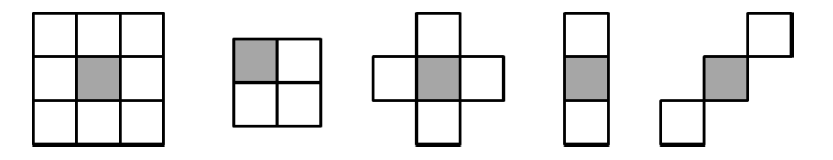
\includegraphics[width=\textwidth/3]{strukturelement.PNG}
\subsection{Erzeugen von Strukturelementen}
Matlab kennt die \lstinline{strel} Funktion um häufige Strukturelemente zu erzeugen.

\subsection{Dilatation}
Bei der Dilatation wird das Strukturelement über das Bild geschoben. Dabei werden alle Referenzpixel eingefärbt, bei welchen das Strukturelement noch ein Pixel des ursprünglichen Bilds berührt.
\begin{lstlisting}
%do a dilation 
ImageDil = imdilate(Image, StrucElem);
\end{lstlisting}

\subsection{Erosion}
Bei der Erosion werden nur diese Referenzpixel erhalten, bei welcher das Strukturelement komplett in die Struktur passt.
\begin{lstlisting}
%do an erosion 
ImageErode = imerode(Image, StrucElem);
\end{lstlisting}

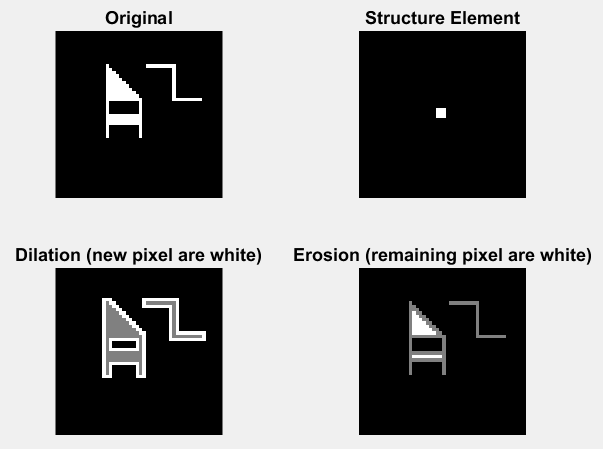
\includegraphics[width=\textwidth/3]{err_dil.PNG}

\subsection{Schliessung und Öffnung}
\begin{description}
    \item[Schliessung] Dilatation und Erosion\\
\begin{lstlisting}
ImageClose = imclose(Image, StrucElem);
\end{lstlisting}
    \item[Öffnung] Erosion und Dilatation
\begin{lstlisting}
ImageOpen = imopen(Image, StrucElem);
\end{lstlisting}
\end{description}

\subsection{Hit- und Miss-Operation}
Ein Strukturelement kann zusätzlich Bedingungen für Nachbarpixel definieren.
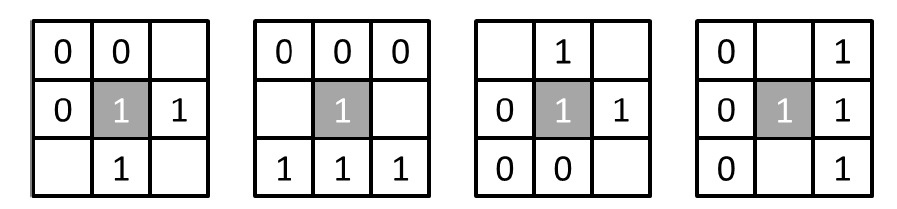
\includegraphics[width=\textwidth/3]{ext_strukturelement.PNG}
wobei:
\begin{description}
    \item[0] Das Pixel muss den Wert 0 haben
    \item[1] Das Pixel muss den Wert 255 (bzw. 1) haben
    \item['' ''] Der Wert dieses Pixels ist irrelevant (wird nicht in Betracht gezogen)
\end{description}
Durch mehrfaches Anwenden eines solchen Strukturelementes entstehen Verdünnungs- (engl. thinning) und Verdickungs-Operationen (engl. thickening).\\
Beispiel: Uebung4/Skeleton.m
\section{Fourier-Transformation}
Die Furier-Transformation erlaubt, ein beliebiges Signal in eine Summe von n Sinussignale zu zerlegen.\\
Einige wichtige Eigenheiten sind:
\begin{itemize}
    \item Das Frequenzspektrum einer aperiodischen Funktion ist kontinuierlich im Intervall $]-\infty , +\infty [$
    \item Das Frequenzspektrum einer periodischen Funktion ist diskret.
\end{itemize}
Da es sich bei Bildern um zweidimensionale Funktionen handelt, wird bei diesen die zweidimensionale Fourier-Transformation verwendet.\\
Definition und Rechenregeln: Skript S. 53.
\subsection{2D Diskrete Fourier Transformation (DFT)}
Die zweidimensionale DFT ist das Produkt der beiden eindimensionalen DFTs.
\begin{lstlisting}
%this is the image size
SizeXImage = 150;
SizeYImage = 150;

%we want to choose power of 2 and have image symmetric
SizeFFT = max(2^ceil(log(SizeXImage)/log(2)), 2^ceil(log(SizeYImage)/log(2)));
%calculate DFT (keep size of image)
Image_FFT = fft2(Image, SizeFFT, SizeFFT);
\end{lstlisting}

\subsubsection{Berechnen der Inversen 2D DFT}
\begin{lstlisting}
%caluclate the inverse fft an plot
Inv_FFT = abs(ifft2(Image_FFT_Mask));
\end{lstlisting}

\subsubsection{Mitteln des Spektrums in Matlab}
Zur Darstellung ist es oft besser, die Spektrumswerte von 0Hz in die Mitte zu verschieben. Dafür kann der Befehl \lstinline|fftshift| verwendet werden.

\subsection{Periodische Strukturen}
Auch die 2D DFT kann verwendet werden, um periodische Strukturen zu finden.
Da ein Bild aber nicht periodisch ist (Ränder), enthält die 2D DFT oft unerwünschte Artefakte. Diese können durch eine künstliche ''Periodisierung'' eliminiert werden.\\
Die einfachste Möglichkeit bietet die Anwendung einer Fensterfunktion (engl. Window Function) welche zum Rand des Bild stetig gegen Null abfällt. Ein bekanntes solches Filter ist das \textbf{Hann-Filter}.
\begin{equation}
w_n=\frac{1}{2}*(1-\cos{\frac{2*\pi *n}{N-1}})
\end{equation}
\begin{lstlisting}
%apply Hanning window
Hann = hann(ImgS(1))*hann(ImgS(2))';
Image_FFT_Ham = fft2(double(Image).*Hann);
\end{lstlisting}

\subsection{Unterdrückung periodischer Strukturen}
Periodische Strukturen/Störungen können in einem Bild durch ein \textbf{Notch-Filter} eliminiert werden.
\begin{lstlisting}
%use imtool to find the positions of the frequencies
%%imtool(log(abs(fftshift(Image_FFT))),[0 log(sum(MaxVal))]);
NotchPos = [107 102; 95 143;116 170; 151 160; 165 114; 143 90; 185 140; 70 118];

%apply the filter 
Filter  = NotchFilter( size(Image_FFT), NotchPos, 6*ones(1,size(NotchPos, 1)) );

%shortcut
ImgS = size(Image);

%do the inverse fft
ImageIfft = abs(ifft2(Image_FFT.*fftshift(Filter)));
%chose only the relevant part
ImageFilt = ImageIfft(1:ImgS(1), 1:ImgS(2));
\end{lstlisting}

\subsection{Alisaing}
Aliasing Artefakte werden häufig durch das Dezimieren (engl. Downsampling) von periodischen Strukturen erzeugt. Durch einen Glättungsfilter können diese stark reduziert werden.
\begin{lstlisting}
DownSampling = 5;   % Downsampling-Faktor

%apply anti aliasing filter
Mask = fspecial('average', 2*DownSampling);
%Mask = fspecial('gaussian', 10*DownSampling, 0.5*DownSampling);

%first apply filter
ImageDecimate = imfilter(Image,Mask);
%do sampling
ImageDecimate = ImageDecimate(1:DownSampling:end, 1:DownSampling:end);
\end{lstlisting}

\subsection{Lineare Filter und DFFT}
Eine Faltung zweier Funktionen im Ortsraum entspricht einer Multiplikation der dazugehörigen DFTs im Ortsfrequenzraum.\\
So können mehrere Filter zusammengefasst werden.
\section{Segmentierung und Merkmalsextraktion}
Unter der Segmentierung eines Bildes versteht man die Zusammenfassung benachbarter Pixel in zusammenhängende Regionen (sog. ,,Regions of Intrest'', ROI).\\
Dafür wird aber ein binäres Bild benötigt, dies kann über eine Schwellwertoperation ermittelt werden.

\subsection{Automatische Schwellwertbestimmung}
Oft wird ein fixer Schwellwert zu ungenügenden Ergebnissen führen. Aus diesem Grund kann die bekannte Methode von \textbf{Otsu} verwendet werden, um den Schwellwert automatisch zu ermitteln. Diese basiert auf folgender Idee:\\
Es wird angenommen, dass das Bild in zwei Klassen von Pixel (mit relativ homogenen Grauwerten) aufgeteilt wird. Die Idee von Otsu ist nun, dass die Verteilung der Grauwerte in den beiden Klassen durch den Schwellwert $K$ derart optimiert wird, dass die Varianzen innerhalb der Klassen möglichst klein sind.\\
Mathematisch:
\begin{align*}
\omega_0 = \sum_{g=0}^{K}p_I(g)\\
\omega_1 = \sum_{g=K+1}^{255}p_I(g)\\
\mu_0 = \frac{1}{\omega_0}\sum_{g=0}^{K}p_I(g)*g\\
\mu_1 = \frac{1}{\omega_1}\sum_{g=K+1}^{255}p_I(g)*g\\
\sigma^2_0 = \frac{1}{\omega_0}\sum_{g=0}^{K}p_I(g)*(g-\mu_0)^2\\
\sigma^2_1 = \frac{1}{\omega_1}\sum_{g=K+1}^{255}p_I(g)*(g-\mu_1)^2\\
\\
\omega_W^2 = \omega_0 * \sigma_0^2 + \omega_1 * \sigma_1^2
\end{align*}
Wobei:
\begin{description}
    \item[$\omega_n$] Wahrscheinlichkeit für Auftreten von Klasse $C_n$
    \item[$\mu_n$] Mittelwert der Klasse $C_n$
    \item[$\sigma_n$] Varianz der Klasse $C_n$
    \item[$\sigma_W$] ''Intra-Klassen'' Varianz
\end{description}
Der optionale Schwellwert ist nun:
\begin{equation}
K_{opt}=argmin(\sigma_W)
\end{equation}
\begin{lstlisting}
%determine image histogram
[Hist, Vals]=imhist(Image);
%normalize it
Hist = Hist/sum(Hist);
%define mean
Mean = Hist.*[0:255]';

%apply Otsu's method
Thresh = [];
%loop over grey values
for Ind = 1:255
    %proability for class 0
    w0 = sum(Hist(1:Ind));
    %proability for class 1
    w1 = sum(Hist(Ind+1:end));
    %mean for class 0
    m0 = sum(Mean(1:Ind))/w0;
    %mean for class 1
    m1 = sum(Mean(Ind+1:end))/w1;
    %store the intra-class probability for this threshold
    Thresh = [Thresh, w0*w1*(m0-m1)^2];
end

%find the maximum value
[MaxThresh, MaxVal]=max(Thresh);
%have to subtract one because we used the index of [0 255]
Threshold = MaxVal-1;
\end{lstlisting}
Oder mit den Matlabeigenen Otsu Funktion:
\begin{lstlisting}
[counts,x] = imhist(I,16);
T = otsuthresh(counts);
BW = imbinarize(I,T);
\end{lstlisting}
\subsubsection{Segmentierung bei nicht globalen Schwellwert}
Das Otsu Verfahren funktioniert aber nur, wenn ein globaler (d.h. für das gesamte Bild konstanter) Schwellwert existiert.\\
Falls dies nicht der Fall sein sollte, gibt es eine Möglichkeit vor der Segmentierung die Grundhelligkeit des Bildes zu extrahieren und vom Originalbild zu subtrahieren.
\begin{lstlisting}
%apply a smoothing filter (we have to know the approximate size of
%forground objects)
Mask = fspecial('gaussian', 40, 25);

%first apply filter
ImageFilt = imfilter(Image, Mask, 'symmetric'); %choose symmetric boundary conditions

%subtract the filtered image from the orginal image; 
Diff = (double(Image)-double(ImageFilt));
%everything below could be done in double; but we want to keep standard 8-bit
%images and have to shift the difference; this can be obtained with 1D histogramm:  
[Hist, Vals] = hist(Diff(:));
Diff = uint8(Diff-Vals(1));

%Use Diff for segmentation
\end{lstlisting}

\subsection{Beschreibung der ROIs (Region of interest)}
Eine genaue Beschreibung der ROI-Methode ist im Skript auf Seite 67 zu finden.\\
Für das Finden der Region of Intrest gibt es hauptsächlich zwei Methoden:
\begin{description}
    \item[Region Labeling] Beim Region Labeling wird das Ganze Bild iteriert und jedes Objekt mit einem Index versehen. Falls ein Nachbarpixel bereits einen Index enthält, wird dieser übernommen, ansonsten um 1 erhöht. Am Schluss wird nochmals iteriert um allfällige Detektionsfehler zu finden.
    \item[Kettencodes] ToDo
\end{description}
\begin{lstlisting}
%do labeling (use 8 neighbors, the default)
[LabelImage, NumberLabels] = bwlabel(Image);
\end{lstlisting}

\section{Merkmalsextraktion}
Die Merkmale von ROIs können mit der Matlab Funktion \lstinline|regionprops()| extrahiert werden.\\
Die zugrundeliegende Mathematik ist im Skript auf Seite 70 ff. aufzufinden.
\begin{lstlisting}
%do feature extraction 
Prop = regionprops(LabelImage,'Area','Centroid', 'Orientation', 'BoundingBox', 'ConvexHull');
%the result is the structure array Prop, with NumLabels x 1 entries
\end{lstlisting}


\section{Liniensegmentierung und Merkmalsextraktion}
Die Liniensegmentierung ist ein Spezialfall der normalen Segmentierung.\\
Die Kantendetektion nach Prewitt und Sobel liefern oft ungenügende Ergebnisse:
\begin{enumerate}
    \item Die Kanten sind in der Regel deutlich breiter als ein Pixel (unnötige Redundanz)
    \item Die Wahl eines globalen Schwellwerts ergibt nicht in allen Bildbereichen eine zufriedenstellende Resultate. Kanten treten oft zu häufig auf oder sie werden erst gar nicht detektiert. Auch ist der Schwellwert manuell.
    \item Zusammengehörende Kanten sind oft, vor allem bei hohen Schwellwerten, unterbrochen.
\end{enumerate}

\subsection{Canny-Algorithmus}
Ein sehr allgemeiner Formalismus, welcher die obigen Probleme löst (mit Ausnahme der Schwellwertwahl) ist der sogenannte Canny Algorithmus.\\
Die Schritte des Canny-Algorithmus:
\begin{enumerate}
    \item \textbf{Glättung:}\\
    Glättung des Bildes mittels eines Gauss Filters.
    \item \textbf{Kantenfilter:}\\
    Anwendung eines Standard Kantenfilters (Sobel, Prewitt) zur Bestimmung des Betrags und der Richtung des Gradienten in jedem Bildpunkt.
    \item \textbf{Bestimmen der lokalen Maxima:}\\
    Basierend auf der Richtung des Gradienten wird für jeden Bildpunkt ermittelt, ob es sich um ein lokales Maximum handelt. Hierzu wird die Änderung der Grauwerte entlang der Richtung des Gradienten betrachtet und das Pixel nur dann selektiert, wenn es einen Gradienten Betrag grösser als die Nachbarpixel hat.
    \item \textbf{Kantenextraktion:}\\
    Hier werden die eigentlichen Kanten selektiert. Dafür wird ein manueller Schwellwert für den Betrag des Gradienten gesetzt. Wird ein Pixel gefunden, dass diesen Schwellwert überschreitet, werden alle Pixel welche diesem lokalen Maximum folgen und einem unteren Sollwert nicht unterschreiten zur Kante hinzugefügt.\\
    Dies ermöglicht eine gute Reaktion auf Kontrastschwankungen.
\end{enumerate}
\begin{lstlisting}
%u7 GradientCanny
%upper and lower threshold for edge detection (relative to max gradient
%value)
Threshold = [0.0 0.05];
%width of Gaussian
Sigma = 1;
%apply a certain threshold
[EdgeCanny, Threshold] = edge(Image,'canny', Threshold, Sigma);
\end{lstlisting}

\subsection{Hough-Transformation}
Einen Punkt/Linie kann auch durch einen Winkel und einen Betrag beschrieben werden (siehe Vektoren, komplexe Zahlen). Bei der Hugh-Transformation wird beim differenzierten Bild jeder Pixel über einen Winkel und Betrag beschrieben. So können zusammenhängende Punkte/Linien ermittelt werden.
\begin{lstlisting}
%u7 HoughTrans
% Detect the edges, the result is a binary image
EdgeCanny = edge(Image, 'canny', [0 0.1], 1);

% Hough transformation, calculate the accumulator Hough
[Hough, Alpha, Rho] = hough(EdgeCanny,'RhoResolution', 2,'Theta',-90:2:89.5);

% Find at most 5 peaks with threshold 15 and minimim distance of 15, 15
% pixel
NumPeaks = 5;
HoughPeaks = houghpeaks(Hough, NumPeaks,'Threshold',5,'NHoodSize',[15,15]);

% Find the lines that correspond to the peaks; fill gabs of 15 pixel and
% suppress all (merged lines) that have a length less than 30 pixel
Lines = houghlines(EdgeCanny, Alpha, Rho, HoughPeaks, 'FillGap', 15, 'MinLength', 50);
\end{lstlisting}

\subsubsection{Prüfen ob Pixel links oder rechts einer Linie liegt}
\begin{lstlisting}
rho_calc = X * cosd(theta) + Y * sind(theta);
if rho_calc > rho
    %Pixel (X,Y) is more right than (rho, theta)
end
\end{lstlisting}

\section{Farbe}
\subsection{Farbräume}
Farben können in verschiedenen Farbräumen dargestellt werden. Dabei unterscheidet man hauptsächlich zwischen Additiven und Substraktiven Farbräumen.
\subsubsection{RGB}
Der RGB (Rot, Grün, Blau) Farbraum ist ein additiver Farbraum in welchem durch Mischen der Farben Rot, Grün und Blau (fast) jede beliebige Farbe erzeugt werden kann.\\
Der RGB-Farbraum wird hauptsächlich zur Bildaufnahme und Wiedergabe an LCD/LED-Monitoren verwendet. Matlab speichert die Farbwerte in einem 3x255-Array.
\begin{lstlisting}
%do a three 3 representation
%extract color planes
Red = Image(:,:,1);
Green = Image(:,:,2);
Blue = Image(:,:,3);
\end{lstlisting}

\subsubsection{CMY}
Für nichtstrahlende Oberflächen können keine additiven Farbräume verwendet werden, da diese selbst keine Wellen aussenden sondern diese nur absorbieren. Dafür werden Cyan, Magenta, Yellow als Filterfarben verwendet.\\
Dieser Farbraum spielt vor allem in der Drucktechnik eine grosse Rolle. Da aber durch die Mischung kein tiefes Schwarz erreicht werden kann, wird als vierte Farbe noch Schwarz hinzugenommen.\\
Die Umwandlung von RGB zu CMYK
\begin{equation}
\begin{bmatrix}
C\\
M\\
Y
\end{bmatrix} =
\begin{bmatrix}
1\\
1\\
1
\end{bmatrix} - 
\begin{bmatrix}
R\\
G\\
B
\end{bmatrix}
\end{equation}

\subsubsection{YCbCr}
Ein weiterer Farbraum ist der YCbCr Farbraum. Dieser hat, nebst vielen anderen Farbräumen die Eigenschaft die Luminanz- (Helligkeits-)(Y) von der Chrominanz- (Farb-)(CbCr) Werten zu trennen. (Formel zur Berechnung auf Skript S. 92)
\begin{lstlisting}
%transform to YCbCr space
ImageYCbCr = rgb2ycbcr(Image);

%extract color planes
Y = ImageYCbCr(:,:,1);
Cb = ImageYCbCr(:,:,2);
Cr = ImageYCbCr(:,:,3);
\end{lstlisting}
\section{Matlab Befehle}
\subsection{Code}
\begin{lstlisting}
%255 --> weiss 
%0 	--> schwarz

%open Image
Image = imread('Image.jpg'); 

%RGB to YCbCr
ImageYCbCr= rgb2ycbcr(ImageRGB);

%subplot 2 hoch 3 breit
figure(1);
subplot(2,3,1);
title('Titel Von Dem Bild'); 
imshow(im1);
subplot(2,3,2);
imshow(im2);
\end{lstlisting}

\subsection{Logical Operations}
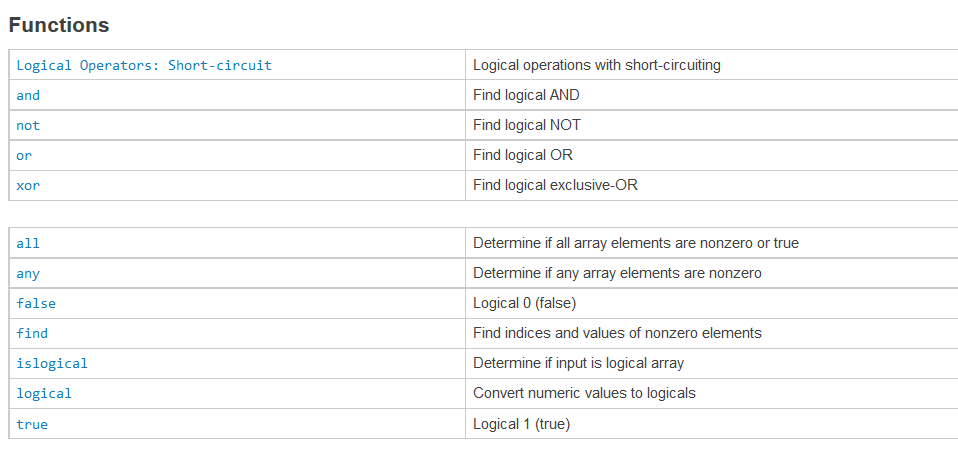
\includegraphics[width=\textwidth/3]{logic_operations.png}

\end{multicols}
\end{document}